\chapter{Introduction to Machine Learning}
Chapter based on UIUC CS 498 Fall 2020 8/26 Lecture: \url{http://slazebni.cs.illinois.edu/fall20/}\\

\section{History of AI Techniques}
\paragraph{Old Techniques}
Before statistical learning, `old-fashioned AI' was the norm. The main idea was to program expertise into the agent. For example, to build a translator using old AI techniques, one would incorporate many different language rules based on experts. This would require putting in many different rules for each type of word, for each type of sentence for each language. While there was some success with such expert engines, they generally never worked. 

\paragraph{Statistical Learning}
Instead of creating expert agents, the modern idea was to program the agent the ability to improve performance based on experience. The agent should be able to gain `experience' from training data or demonstrations. This technique is much more flexible. For example, to build an expert agent to recognize an everyday object like a chair, one would have to come up with a specific definition that generally fits all chairs. Alternatively, using statistical learning techniques, we can show an agent many examples of different types of chairs and the agent can `learn' what defines a chair without a human having to actually define it. By learning, we mean that we want to optimize the performance of the agent on training data and then hope that it \textit{generalizes} to unseen examples. This `generalization' is not theoretically given and is a current area of research. 

\section{General Learning Procedure}
\paragraph{Learning Pipeline}
Training samples --> Feature Extraction --> Training --> Learned Model \\
The general learning procedure first starts off with a group of training samples (not necessarily labelled). Historically, before the actual training begins, some type of \textit{feature extraction} has to take place. Feature extraction usually involves some type of transformation of the data into the input form that goes into model. For example, a form of feature extraction for natural language processing could involve removing commonly used words. After the feature extraction takes place, the training process takes place and the result is the learned model. To test the quality of the learned model, the model is evaluated (the input is passed through the model without `saving' any of the information from the test data) on a test set which includes data that the model has not seen before during training. 

\paragraph{Basic Supervised Learning Framework}
Mathematically, the framework described above can be seen as follows: $y = f(x)$ where $y$ is the output, $f$ is the prediction function and $x$ is the input. Training or learning means given a training set of labelled examples $\{(x_1,y_1), \dots, (x_n,y_n)\}$, a predictor $f$ is created. Testing means applying $f$ to a new test example $x$  and output the predicted value $y$. 


\section{Simple Classification Models}
\paragraph{Nearest Neighbor Classifier}
Training points are labelled with a class. The label of a test point is the label of the training example nearest to the test point. Nearest can mean Euclidean distance, Manhattan distance, etc.  This is a simple classifier since it only needs the distance function and no training is required. A variant of nearest neighbor, is $k$-nearest neighbor where for a new point, find the $k$ closet points from training data. Higher $k$-nearest neighbor is generally more robust to outliers and can create more complex decision boundaries as shown in the image below.
\begin{figure}
\caption{k=1 vs k=5 nearest neighbors}
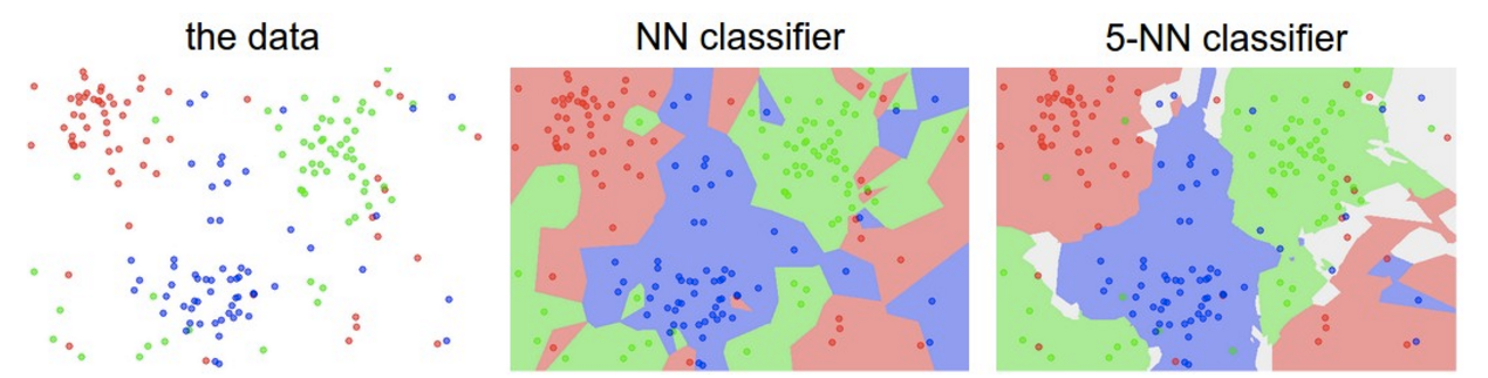
\includegraphics{nearest_neighbor}
\end{figure}
Nearest neighbor methods does have many limitations. An example of running k-nearest neighbors on pixels of images is seen below.
\begin{figure}
\caption{Nearest neighbor on images. A simple distance metric does not capture the real differences between images. One would have to engineer a quite complicated distance function to accurately use nearest neighbor for images. It is easier to learn functions that represent the images.}
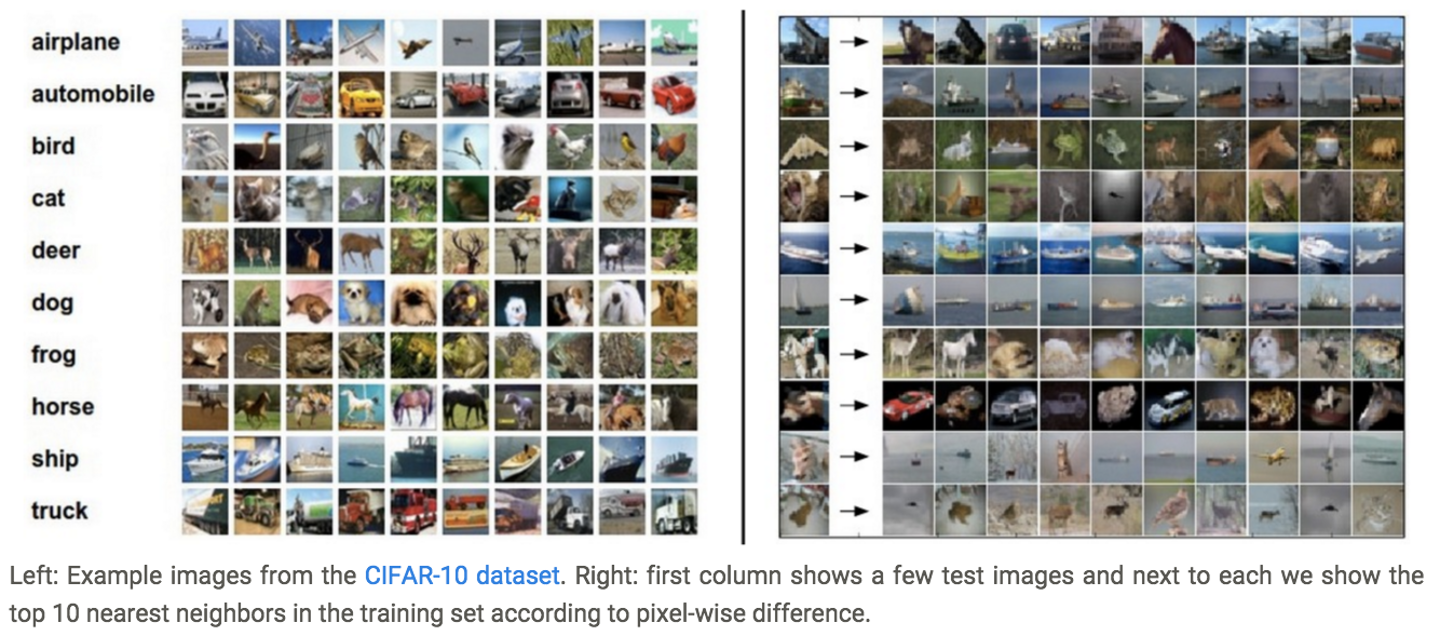
\includegraphics{cifar_nearest_neighbor}
\end{figure}
\paragraph{Linear Classifier}
For linear classifiers, we want to find a linear function to separate the classes. Linear classifiers are parametric meaning there are parameters that represent the (ideally a compressed form of) training data. Linear classifiers have as many parameters as training points. Each training point $x_i$, has a weight $w_i$. To determine where classes are separate (note that this linear classifier can only handle two classes), we use the following parametric equation to identify a hyperplane:
$f(x) = sgn(w_1x_1 + w_2x_2 + \dots + w_Dx_D +b) = sgn(w \dot x +b)$. Points that are one side of the hyperplace are classified as one class and points on the other side are classified as the other. Note that there will be `mis-classified' points whose actual label is different than the label assigned by the classifier. \\

At this point we have not discussed how we learn the parameters of the linear classifier. Learning parameters of different models will be the subject of many of the next chapters. 

\paragraph{Pros and Cons of Nearest-Neighbor and Linear Classifiers}
Pros of nearest neighbor methods include that it is simple to implement, decision boundaries are not necessarily linear, works for any number of classes and it is a nonparametric method (no parameters to learn). The cons are that it requires are good distance function and is slow. Linear classifier pros include that it is a low-dimensional parametric representation and is very fast at test time. Cons are that it only works for two classes, we have to train the classifier and if the data are not linearly separable (we cannot draw a straight line through the data) then the method is not accurate (we will expand on this later).

\section{Taxonomy of Statistical Learning Problems}
Classification is a form of \textit{supervised} learning, where we are given the labels for our training data. Regression and structured prediction are also forms of supervised learning. The difference between these three problems is the form of the output. Classification output is discrete (like names of animals), regression output is continuous and structured prediction has complicated structures like parsing trees. 
\paragraph{Supervised Learning}
So far we have seen classification, where the output values we are predicting are discrete. In \textbf{Regression} problems, the output values are continuous. In \textbf{structured prediction}, the outputs are more complicated structures like parsing trees. 
\paragraph{Unsupervised Learning}
\textit{Unsupervised} learning is a situation where there is unlabelled data as input and the goal is to learn some structure of the data. The goal is less clearly defined than in supervised learning. Examples of unsupervised learning include clustering, where the goal is try to find 
groups of similar data points, quantization or data compression where the goal is to encode the data into a more compact form, and dimensionality reduction where the goal is to discover a lower-dimensional surface on which the data lives. Another type of unsupervised learning is concerned with learning the data distribution which can be solved with density estimation (finding a function that approximates the probability density of the distribution and learning to sample where you produce samples that mimic the training distribution. 
\paragraph{Other Forms}
There are forms of learning in-between unsupervised and supervised. \textit{Semi-supervised} learning contains labels for a small portion of the training data and \textit{weakly supervised} has noisy labels or labels are not exactly for the task of interest. In \textit{self-supervised} learning, the model uses part of the data to predict other parts of the data. In \textit{reinforcement learning}, the model learns from rewards in a sequential environment. Reinforcement learning is the learning behind many games. In \textit{active learning}, the learning algorithm can choose its own training examples or ask a `teacher' for an answer on selected inputs.  \textit{Lifelong learning} is focused on learning over time. There are many other subfields of learning but these are some of the major ones. 